%% evaluation.tex
%%

%% ==============================
\chapter{Results}
\label{ch:results}
%% ==============================

To find indications for the ``Heisenberg Effect'' in the collected data, it was important to first take a look at other effects that may occur and had an influence on the accuracy of the pointing tasks. The paper done by Pavlovych and Stuerzlinger~\cite{pavlovych_tradeoff_2009} suggest to take a deeper look on hand tremor and device jitter to precisely analyze effects in distal pointing tasks. 

\section{Clearing the data from disturbing effects}
\label{sec:evaluation:clearing_the_data}

\begin{figure}[h]
    \centering
    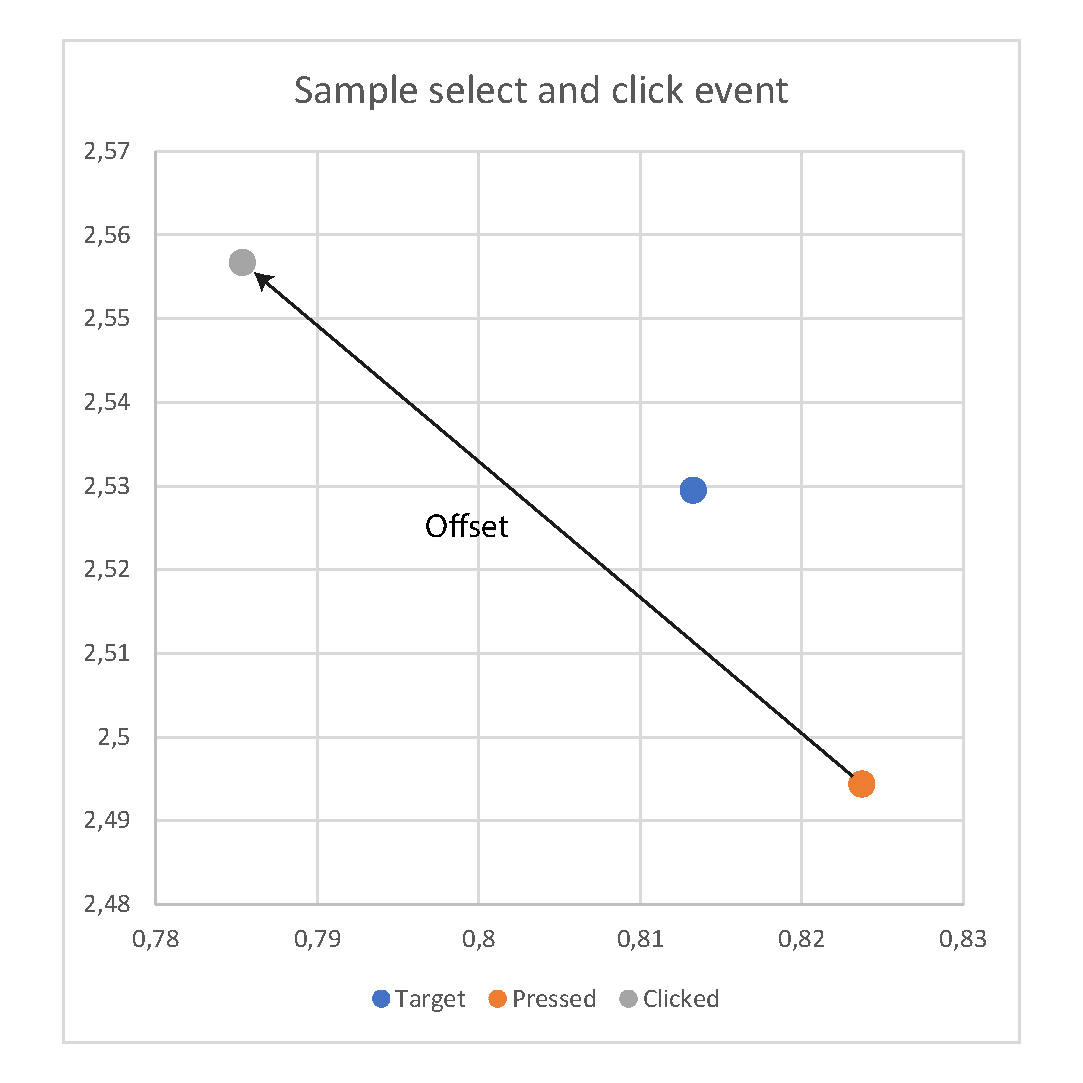
\includegraphics[width=.45\columnwidth]{graphics/graphs/sample_point_and_click_event_edited.pdf}
    \caption{A single sample from the data. }
    \label{fig:sample_point_and_click_event}
\end{figure}

\subsection{Calculation offset}
\label{subsec:evaluation:clearing_the_data:calculating_offset}

To clear the data from disturbing effects, it was important to analyze the overall offset at first. With offset, it is meant the distance between the position of the cursor, where the user first slightly pressed the trigger (a slight press is not activating a click event. The trigger has to be fully pressed in), and the position of the cursor, when the user clicked and hit the target. It was to suspect, that in this offset, the ``Heisenberg Effect'' can be found. For illustration, Figure~\ref{fig:sample_point_and_click_event} shows in orange the position when the user first pressed the trigger. The blue dot marks the actual target and the grey dot marks the position where the controller pointed at when the user fully clicked the trigger. The distance between the pressed position and the clicked position is the described offset.

\subsection{Device-caused jitter}
\label{subsec:evaluation:clearing_the_data:device_caused_jitter}

As mentioned in Subsection~\ref{subsec:basic_jitter}, the jitter caused by the controller and the VR headset were tracked while both devices weren't moved at all. The controller was placed on the floor and the headset on a table. The tracked positions showed a small fluctuation in the position reporting of the devices. With the saved positions a maximum and minimum of these fluctuations were calculated and set in perspective with the other effects. In Figure~\ref{fig:static_device_jitter_compared_to_offset} is shown how minimal the effect of the jitter based on the devices is, compared to the overall offset. The offset is in this figure, the difference between the point the user is first pressing the button to select a target, and the position the click event is tracked.

\begin{figure}[h]
    \centering
    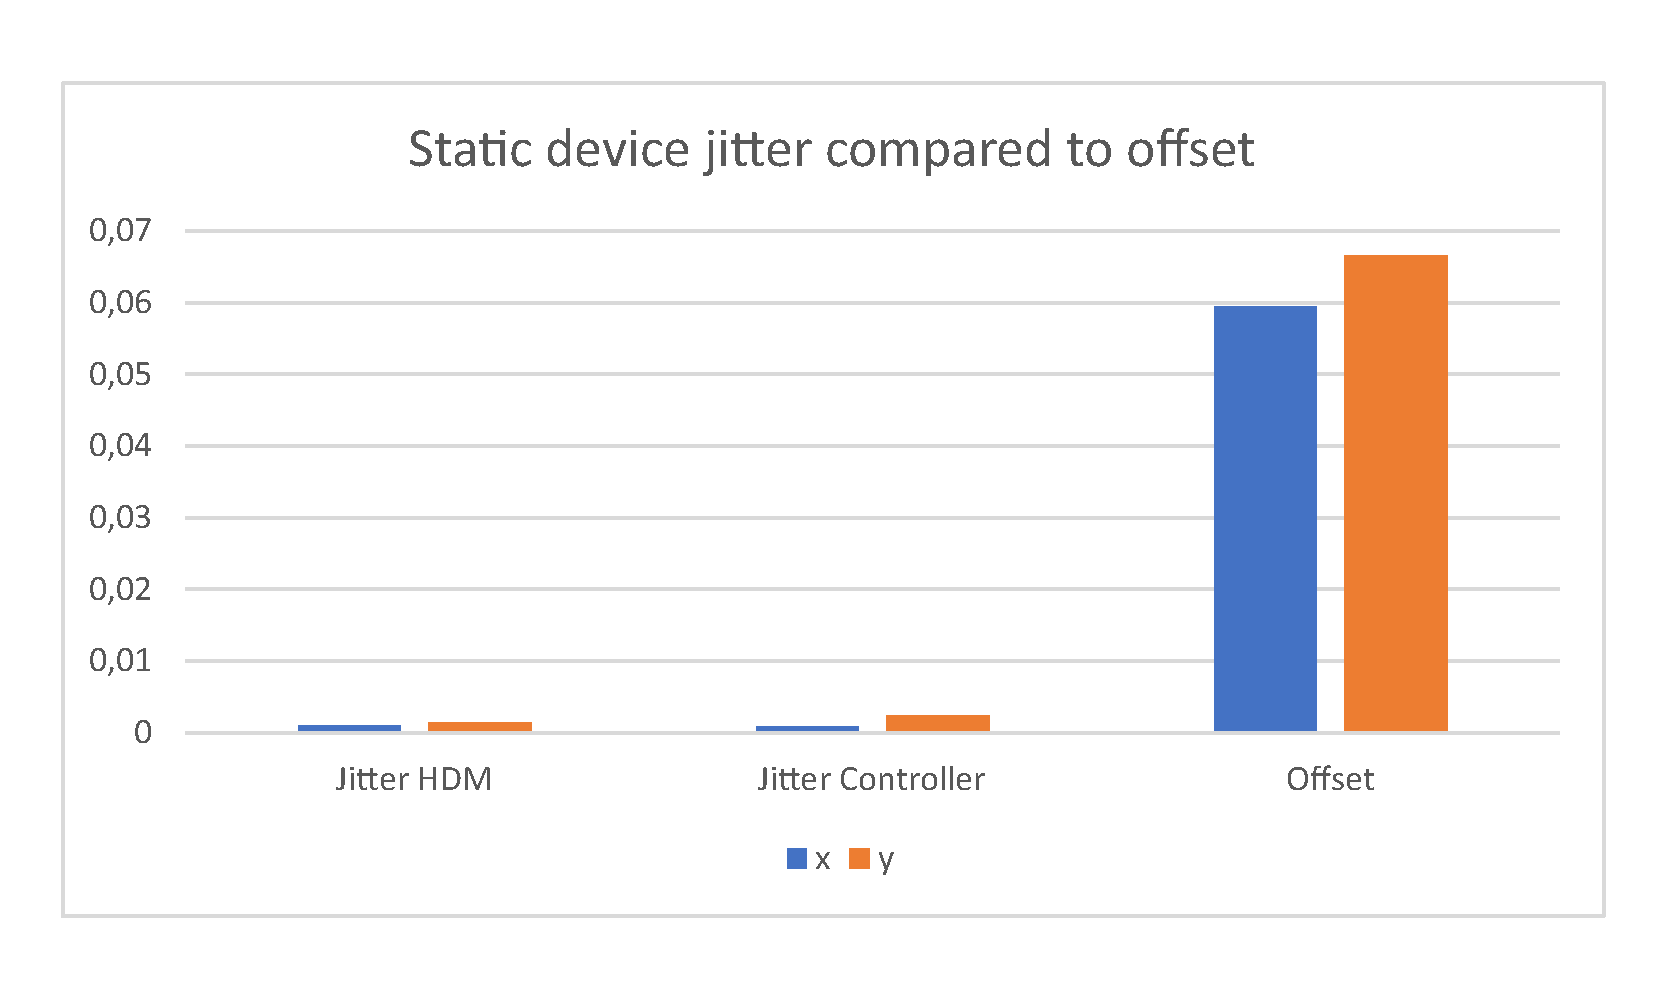
\includegraphics[width=.9\columnwidth]{graphics/graphs/static_device_jitter_compared_to_offset.pdf}
    \caption{Static jitter of the devices compared to the actual offset between intention to click and result hit on the target}
    \label{fig:static_device_jitter_compared_to_offset}
\end{figure}

\subsection{Hand tremor}
\label{subsec:evaluation:clearing_the_data:hand_tremor}

To determine the effects of hand tremor to the data, the changes in position were tracked, when users had to hold still in the target for finishing the timer. These fluctuations were plotted over all tasks. Tasks are here the different stages of the procedure: to stand up/sit down, to stretch the arm out/apply it to the body and the degrees of freedom given to the controller. The data for the offset was also distributed over these tasks and set in comparison to the data calculated as the hand jitter. The result is shown in Figure~\ref{fig:difference_handjitter_offset}. The figure shows clearly, that hand tremor has an impact on the accuracy of the pointing but can't be declared as the main reason for the offset. It is also shown, that with the arm stretched out hand tremor increases as expected.  

\begin{figure}[h]
    \centering
    \includegraphics[width=.9\columnwidth]{graphics/graphs/difference_handjitter_offset.pdf}
    \caption{Difference between offset by hand tremor and overall offset plotted over all different tasks}
    \label{fig:difference_handjitter_offset}
\end{figure}

\section{Indications for the Heisenberg Effect}
\label{sec:evaluation:indications}

\begin{figure}[h]
    \centering
    \includegraphics[width=.75\columnwidth]{graphics/graphs/final_plot.pdf}
    \caption{Combination of all targets and results}
    \label{fig:plot}
\end{figure}

After clearing the data and setting it in comparison with other effects, it is clear, that hand tremor and device jitter aren't the main reasons for the offset between aimed position and hit position in the collected data. The results suggest, that the, first by Bowman~\cite{bowman_using_2001} mentioned, ``Heisenberg Effect'' is the reason for this offset. 
\newline
\newline
If all data is plotted together, the effect gets even clearer. A look at Figure~\ref{fig:plot} shows, that the offset has one direction, upwards. The blue dots symbolize the targets on the Fitt's Law based circle (as explained in detail in subsection~\ref{subsec:impl:circle_task}), and the green and red dots symbolize the final position of the hit, when the click was tracked (green are the positions with 3DOF and red are the positions with 6DOF). Hand tremor and device jitter would have caused balanced ``hit fields'' around the targets. The collected data suggest, that the effects of hand tremor and jitter result in a normal distribution around the targets. But as the Figure shows, all hits are above the target. This suggests the conclusion, that the up going movement of the click, is resulting in this offset. 